\chapter{Progetto e attività di stage}
\textit{Questa capitolo parla delle attività di stage andando a descrivere il progetto nei suoi stati di avanzamento, le scelte adottate e le motivazioni che mi hanno permesso di scegliere.}

\section{Formazione}
All'inizio dello stage, la prima attività che ho dovuto svolgere è stata quella di studio delle applicazioni adottate dall'azienda e i formalismi, ovvero codici e abbreviazioni adottate per la realizzazione dei campi di database. 
Per la formazione sull'applicazione \inde\, ho seguito sei video-corsi della durata di una o anche due ore l'uno. In aggiunta, per velocizzare l'apprendimento dell'uso dell'applicazione, è stato richiesto che venissero realizzate le applicazioni presenti nei video.
Rispetto a quanto pianificato, l'apprendimento del programma è risultato più rapido della settimana preventivata e quindi, durante la stessa, ho potuto interfacciarmi con i data warehouse e lo studio di alcune stored procedure. 
Verso fine settimana ho iniziato lo studio dei documenti relativi al configuratore catalogo/prodotti.


\section{Progettazione logica e architetturale}
Dalla seconda settimana di stage, ho iniziato ad affrontare le dinamiche aziendali concentrandomi nelle attività di progetto che è stata divisa in incontri con il cliente e lavoro presso la sede di Castelfranco.

\subsection{Database}
Affiancato al tutor aziendale, il primo punto affrontato è stato il database. Il cliente ci ha dato carta bianca, ovvero potevamo decidere tra due soluzioni: riutilizzare tabelle presenti nel database oppure crearne di nuove. Questo cliente specifico dispone tra i suoi software di sei applicazioni ideate con InDe e nei mesi di stage hanno iniziato a chiedere nuovi progetti.

La scelta, dopo una attenta discussione con il cliente, è stata quella di creare delle tabelle nuove perché questa nuova componente in futuro vorrebbero integrarla in altre applicazioni oltre che a quella per cui è stata realizzata.\\
Per cercare di mantenere una certa uniformità con il resto del data warehouse, la prima scelta è stata quella di non inserire vincoli di Foreign Key.
Questo vincolo che avrebbe permesso query più rapide è risultato superfluo in seguito alla velocità dei server. Tuttavia, continuo a ritenere molto utile la creazione delle foreign key perché in questo modo se anche le tabelle iniziano ad avere una quantità di record spropositata la velocità resta soddisfacente. Inoltre, il problema dell'eventuale plugin dell'applicazione richiede comunque che si metta mano al codice nell'importazione della componente. 
Quest'ultima scelta ha portato il vantaggio di estendere i progetti in maniera più rapida.
Infine, per concludere il tema vincoli gli unici adottati sono quelli di Primary Key.
\\

La prima tabella da cui partire è quella dedicata agli articoli. Quest'ultima è già presente nel data warehouse e dispone di una vista. Partendo da questi due contenitori, si è realizzata una struttura che permetta prima di realizzare una lista prodotti, poi, se l'articolo esiste, arricchire le sue informazioni.\\

Gli aspetti da tenere in considerazione sono stati:
\begin{itemize}
	\item ogni articolo ha delle immagini, video o dei file di vario genere;
	\item ogni articolo deve poter avere uno o più tag;
	\item ogni articolo deve avere delle informazioni di base e delle informazioni aggiuntive;
	\item ogni informazione aggiuntiva deve poter essere gestita (creata, modificata ed eliminata).
\end{itemize}
Queste informazioni sono state definite durante la prima riunione presso la sede del cliente.\\

\begin{figure}[!h] 
	\centering 
	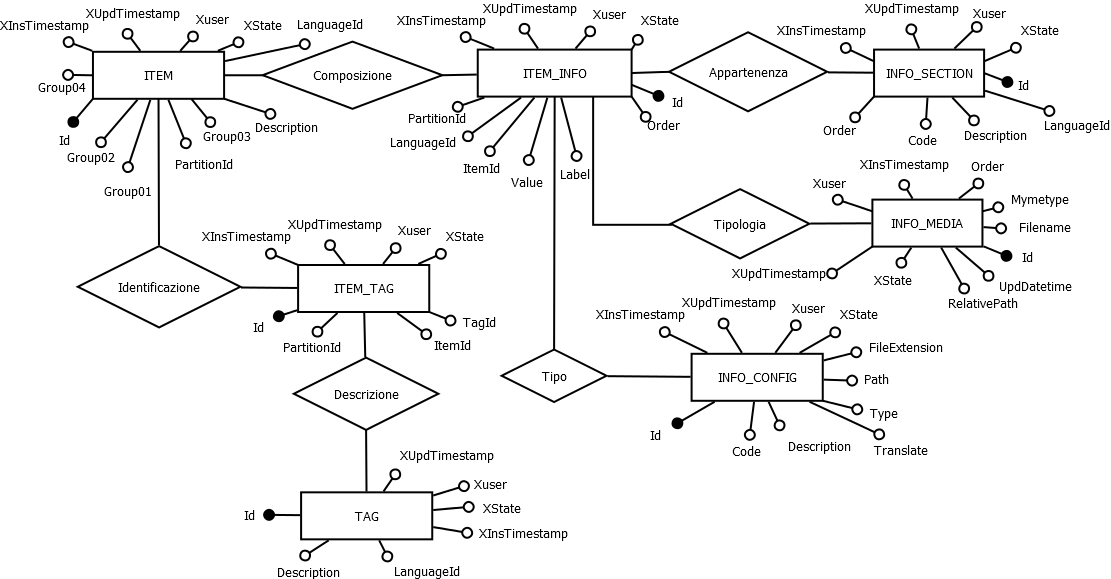
\includegraphics[width=1\columnwidth]{DiagrammaER} 
	\caption{Diagramma Entity Relationship}
	\label{DiagrammaER}
\end{figure}

Il diagramma ER (i vincoli sono fittizi, mostrano i collegamenti nonostante l'assenza di foreign key) è stato pensato in modo tale che ogni articolo dispone di molte informazioni e ciascuna di esse appartiene ad una categoria.

\paragraph{ITEM}
Questo oggetto è una vista con alcune delle informazioni più importanti. Visto che la fase di inserimento prevede unicamente che un'utente possa inserire alcune informazioni. I dati gestiti nella vista sono i gruppi di appartenenza (ad esempio insaccati, surgelati, prodotti da forno) ed una descrizione breve dell'oggetto.
In questo contesto la descrizione appare due volte una negli ITEM ed una nella ITEM\_INFO per il semplice motivo che la tabella esisteva già nel database.

\paragraph{ITEM\_INFO}
Nella seguente tabella vengono raccolte tutte le informazioni e rappresenta il punto di collegamento dell'intero progetto. In esso vengono inserite le etichette e i valori che rappresentano i punti fondamentali di questa tabella. Le etichette (label) sono la descrizione dei valori (value) che permettono ricerche in tabella più rapide (video, titolo, immagine). I valori sono quelli che in base alle altre tabelle saranno stampati a video dall'applicazione web di front-end (\hyperref[frontend]{figura \ref{frontendad}}).

\paragraph{INFO\_CONFIG}

\paragraph{INFO\_MEDIA}

\paragraph{INFO\_SECTION}

\paragraph{TAG}

\paragraph{ITEM\_TAG}



\subsection{Design Pattern}
Facade spiegare perchè adottato e come si è pensato di realizzarlo
UML

\section{Progettazione di dettaglio}
Quali sono le ulteriori attenizoni a cui bisogna fare attenzione se ce ne sono.
UML, comportamento delle funzionalità principali


\section{Codifica}
Spiegare le singole attività svolte per ogni singolo oggetto (i più importanti )

\subsection{Classi}

\subsubsection{Classi di base}

\subsubsection{Facade: CatalogoProdotto}


\subsection{Videate}
elenco delle videate normali

\subsubsection{Modali}
metodo seguito come le si sono implementate


\section{Verifica, validazione e collaudo}


\section{Altri interventi}



